%==============================================================
%  RecaLL -- Diagram Book
%  Every diagram of the final report, one per page, at full size.
%  Figure numbers are the same as in the report (main.tex).
%  Uses the same preamble, cover data and image files as the report.
%  Build: latexmk -pdf diagrams.tex
%==============================================================
\documentclass[12pt,a4paper]{report}

%==============================================================
%  preamble.tex -- packages, colours, helper macros.
%  Students normally DO NOT need to edit this file.
%==============================================================
\usepackage[T1]{fontenc}
\usepackage[utf8]{inputenc}
\usepackage[a4paper,margin=1in,headheight=26pt]{geometry}
\usepackage{setspace}
\onehalfspacing
\IfFileExists{lmodern.sty}{\usepackage{lmodern}}{}
\usepackage[expansion=false]{microtype}

% ---- graphics, colours, tables ---------------------------------
\usepackage[dvipsnames,table]{xcolor}
\usepackage{graphicx}
\graphicspath{{images/}{images/diagrams/}{images/photos/}}
\usepackage{float}
\usepackage{booktabs,array,tabularx,longtable,multirow,makecell}
\usepackage{etoolbox}
% Slightly tighter line spacing inside long tables (body text stays one-and-a-half spaced).
\AtBeginEnvironment{longtable}{\setstretch{1.1}}
\usepackage{caption,subcaption}
\captionsetup{font=small,labelfont=bf}
\usepackage{enumitem}
\setlist{itemsep=2pt,topsep=3pt}
\usepackage{amsmath,amssymb}
\usepackage{pifont}
\newcommand{\cmark}{\ding{51}}   % tick mark for contribution / traceability tables
\usepackage{pdflscape}           % \begin{landscape} for wide tables / diagrams
\usepackage[figuresright]{rotating} % sidewaysfigure for \widefig

% ---- CUET colour palette ---------------------------------------
\definecolor{cuetblue}{RGB}{38,36,115}
\definecolor{cuetgold}{RGB}{218,165,32}
\definecolor{cuetgreen}{RGB}{34,139,34}

% ---- diagrams / Gantt ------------------------------------------
\usepackage{tikz}
\usetikzlibrary{shapes,arrows.meta,positioning,fit,calc}
\usepackage{pgfgantt}
\usepackage{pgfplots}
\pgfplotsset{compat=1.18}

% ---- code listings ---------------------------------------------
\usepackage{listings}
\lstdefinestyle{cuetcode}{
  basicstyle=\ttfamily\footnotesize,
  keywordstyle=\bfseries,
  commentstyle=\color{black!60}\itshape,
  stringstyle=\color{black!80},
  numbers=left, numberstyle=\tiny\color{gray}, numbersep=6pt,
  frame=single, rulecolor=\color{gray!60},
  breaklines=true, breakatwhitespace=false,
  showstringspaces=false, tabsize=4, captionpos=b,
  backgroundcolor=\color{gray!5}}
\lstset{style=cuetcode}
\renewcommand{\lstlistingname}{Listing}

% ---- algorithms (pseudocode for LLD) ---------------------------
\usepackage{algorithm}
\usepackage{algpseudocode}

% ---- headers / footers -----------------------------------------
\usepackage{fancyhdr}
\pagestyle{fancy}
\fancyhf{}
\fancyhead[L]{\small\textcolor{cuetblue}{Project Report}}
\fancyhead[R]{\small\textcolor{cuetblue}{\CourseCode}}
\fancyfoot[C]{\thepage}
\renewcommand{\headrulewidth}{0.4pt}
\renewcommand{\headrule}{\hbox to\headwidth{\color{cuetgold}\leaders\hrule height \headrulewidth\hfill}}
\fancypagestyle{plain}{\fancyhf{}\fancyfoot[C]{\thepage}\renewcommand{\headrulewidth}{0pt}}

% ---- chapter / section title colours ---------------------------
\usepackage{titlesec}
\titleformat{\chapter}[display]
  {\normalfont\huge\bfseries}
  {\chaptertitlename\ \thechapter}{10pt}{\Huge}
\titlespacing*{\chapter}{0pt}{-20pt}{25pt}
\titleformat{\section}{\normalfont\Large\bfseries\raggedright}{\thesection}{1em}{}
\titleformat{\subsection}{\normalfont\large\bfseries}{\thesubsection}{1em}{}

% ---- guide boxes (toggle in config.tex) ------------------------
\usepackage[most]{tcolorbox}
\newif\ifguides
\newcommand{\guide}[1]{%
  \ifguides
    \begin{tcolorbox}[colback=blue!4,colframe=cuetblue,boxrule=0.6pt,arc=2pt,
      left=4pt,right=4pt,top=2pt,bottom=2pt,title={\small\bfseries GUIDE (delete before submission)}, fonttitle=\small]
      \small #1
    \end{tcolorbox}
  \fi}

% ---- figure helper: prints a placeholder if the image is missing
% Usage: \figplaceholder{file}{caption}{label}[width]
\newcommand{\figplaceholder}[4][0.85\textwidth]{%
  \begin{figure}[htbp]\centering
    \IfFileExists{images/diagrams/#2}{\includegraphics[width=#1,height=0.78\textheight,keepaspectratio]{#2}}%
    {\IfFileExists{images/#2}{\includegraphics[width=#1,height=0.78\textheight,keepaspectratio]{#2}}%
    {\fbox{\parbox{#1}{\centering\vspace{2cm}\textcolor{red}{[Figure placeholder: \texttt{\detokenize{#2}}]}\vspace{2cm}}}}}
    \caption{#3}\label{#4}
  \end{figure}}

% ---- wide figure on its own landscape page ------------------------
% Usage: \widefig{file}{caption}{label}  (for diagrams too wide for portrait)
% Rotated float (rotating package): floats to its own page, so the surrounding
% text keeps flowing and no near-empty pages are left behind.
% The page's text height and width are saved before rotation, because inside
% sidewaysfigure \textwidth is replaced by the page height.
\newlength{\rclLong}\newlength{\rclShort}
\AtBeginDocument{\setlength{\rclLong}{\textheight}\setlength{\rclShort}{\textwidth}}
\newcommand{\widefig}[3]{%
  \begin{sidewaysfigure}\centering
    \IfFileExists{images/diagrams/#1}{\includegraphics[width=\rclLong,height=0.86\rclShort,keepaspectratio]{#1}}%
    {\fbox{\parbox{0.8\rclLong}{\centering\vspace{2cm}\textcolor{red}{[Figure placeholder: \texttt{\detokenize{#1}}]}\vspace{2cm}}}}
    \caption{#2}\label{#3}
  \end{sidewaysfigure}}

% ---- team member macros (used by config.tex) -------------------
\makeatletter
\newcommand{\coverlist}{}
\newcommand{\tablerows}{}
\newcommand{\memberphoto}[1]{%
  \IfFileExists{#1}{\includegraphics[width=2cm,height=2.4cm,keepaspectratio]{#1}}%
  {
\includegraphics[width=2cm,height=2.4cm,keepaspectratio]{images/photos/placeholder.png}}}
\newcommand{\member}[7]{%
  \g@addto@macro\coverlist{#1 \quad ID: #2\\[0.5ex]}%
  \g@addto@macro\tablerows{\memberphoto{#7} & #1 & #2 & {\scriptsize\url{#3}} & \mbox{#4} & #5 & #6 \\ \hline}}
\makeatother

% ---- hyperlinks (load LAST) ------------------------------------
\usepackage[hidelinks]{hyperref}
\hypersetup{pdftitle={RecaLL: Software Engineering Final Report}}
\usepackage[nameinlink]{cleveref}

% ---- line breaking for long code names / paths -----------------
% Allow \texttt{} words (file paths, identifiers) to break after / . _ -
\usepackage{xurl}
\emergencystretch=3em
% Let \_ inside \texttt break (paths like app/services/rag_service.py):
\makeatletter
\DeclareRobustCommand{\_}{\ifmmode\nfss@text{\textunderscore}\else\textunderscore\fi\discretionary{}{}{}}
\makeatother

% ---- handy macros ----------------------------------------------
\newcommand{\todo}[1]{\textcolor{red}{\textbf{[TODO: #1]}}}
\newcommand{\req}[1]{\texttt{#1}}

%==============================================================
%  config.tex  --  THE ONLY FILE YOU NEED TO EDIT FOR THE COVER
%==============================================================

% Guide boxes off for the submitted version.
%\guidestrue
\guidesfalse

% --- Project information ----------------------------------------
\newcommand{\ProjectTitle}{RecaLL: An AI-Powered Active Recall Study Desktop App}
\newcommand{\CourseCode}{CSE-356}
\newcommand{\CourseName}{Software Engineering (Sessional)}
\newcommand{\SubmissionDate}{19 November 2026}

% --- Supervisor / course teachers (shown on the cover page) -----
\newcommand{\SupervisorNames}{%
  \textbf{Mir Md.\ Saki Kowsar}\\ Assistant Professor, Department of CSE, CUET\\[0.6ex]
  \textbf{Md.\ Refaj Hossan}\\ Lecturer, Department of CSE, CUET}

% --- Team members ------------------------------------------------
% \member{Name}{ID}{Email}{Contact No.}{Total Credit Passed}{CGPA}{photo file}
% Photos: put JPG/PNG files in images/photos/ named by student ID.
\member{Al Rubayet}{2204002}{u2204002@student.cuet.ac.bd}{+880 1633-707780}{101.75}{3.40}{images/photos/2204002.jpeg}
\member{Md. Rony Hossain}{2204005}{u2204005@student.cuet.ac.bd}{+880 1817-358156}{101.75}{3.50}{images/photos/2204005.jpg}
\member{Imteajul Islam}{2204015}{u2204015@student.cuet.ac.bd}{+880 1749-553050}{101.75}{3.52}{images/photos/2204015.jpeg}
\member{Tahsin Ahmed Chowdhury}{2204028}{u2204028@student.cuet.ac.bd}{+880 1841-230608}{101.75}{3.50}{images/photos/2204028.png}


\renewcommand{\ProjectTitle}{RecaLL: An AI-Powered Active Recall Study Desktop App\\[0.1cm]
  \large Diagram Book}
% The cover is one line taller than the report's, so tighten it slightly.
\renewcommand{\SupervisorNames}{%
  \textbf{Mir Md.\ Saki Kowsar}\\ Assistant Professor, Department of CSE, CUET\\[0.3ex]
  \textbf{Md.\ Refaj Hossan}\\ Lecturer, Department of CSE, CUET}
\fancyhead[L]{\small\textcolor{cuetblue}{RecaLL Diagram Book}}

% ---- one diagram per page -------------------------------------
% Wide diagrams (width > 1.15 x height) are turned sideways on a portrait page.
\newsavebox{\dgbox}
\newcommand{\dgpending}{}
\newcommand{\dgsec}[1]{\gdef\dgpending{#1}}
\newcommand{\dgtoc}[2]{%
  \ifx\dgpending\empty\else
    \phantomsection\addcontentsline{toc}{chapter}{\dgpending}%
    \gdef\dgpending{}%
  \fi
  \phantomsection\addcontentsline{toc}{section}{Figure #1: #2}}
\newcommand{\dghead}[2]{%
  \noindent{\large\bfseries Figure #1.}\enspace{\large #2}\par
  \vspace{0.2cm}\noindent{\color{black!40}\rule{\linewidth}{0.4pt}}\par}
% \dgpage{sideways?}{number}{caption}{content}
% Every page stays portrait (same size and header throughout, prints cleanly).
% Wide diagrams (S) are turned 90 degrees on the portrait page, like the
% sideways figures in the report, so they still use the whole page.
\newcommand{\dgpage}[4]{%
  \clearpage
  \noindent\dgtoc{#2}{#3}%
  \ifx#1S
    \vspace*{\fill}{\centering\rotatebox{90}{\begin{minipage}{0.92\rclLong}
      \dghead{#2}{#3}\vspace{0.3cm}\centering #4
    \end{minipage}}\par}\vspace*{\fill}%
  \else
    \dghead{#2}{#3}%
    \vfill\begin{center}#4\end{center}\vfill
  \fi
  \clearpage}
% \dg{file}{number}{caption}
\newcommand{\dg}[3]{%
  \sbox{\dgbox}{\includegraphics{#1}}%
  \ifdim\wd\dgbox>1.15\ht\dgbox
    \dgpage{S}{#2}{#3}{\includegraphics[width=\linewidth,height=\dimexpr\rclShort-2.4cm\relax,keepaspectratio]{#1}}%
  \else
    \dgpage{P}{#2}{#3}{\includegraphics[width=\textwidth,height=\dimexpr\textheight-2.8cm\relax,keepaspectratio]{#1}}%
  \fi}

\begin{document}

\pagenumbering{gobble}
% Copy of frontmatter/cover.tex for the diagram book, with a smaller logo so the
% extra "Diagram Book" line still fits on one page.
%---------------- Cover page (reads data from config.tex) -------
\begin{titlepage}
\centering
{\Large\bfseries\color{cuetblue} Chittagong University of Engineering \& Technology}
\IfFileExists{images/cuet_logo.png}{
\includegraphics[width=0.27\textwidth]{images/cuet_logo.png}}{\fbox{CUET LOGO}}\par
\vspace{0.25cm}{\large\bfseries\color{cuetblue} Course Code: \CourseCode\par}
\vspace{0.1cm}{\Large\bfseries\color{cuetblue} \CourseName \par}\vspace{0.2cm}
{\color{cuetgold}\rule{0.82\textwidth}{1.5pt}}\par
\vspace{0.25cm}
{\LARGE\bfseries\color{cuetblue} \ProjectTitle\par}
\vspace{0.25cm}
{\color{cuetgold}\rule{0.82\textwidth}{1.5pt}}\par
\vspace{0.3cm}
{\Large\bfseries Team Members\par}
\vspace{-0.1cm}
{\rule{0.32\textwidth}{0.8pt}}\par
\vspace{0.25cm}
\coverlist
\vspace{0.2cm}
{\large\bfseries\color{cuetblue} Supervised by\par}
\SupervisorNames\par
\vspace{0.25cm}
{\SubmissionDate\par}
\vfill
{\color{cuetgold}\rule{0.9\textwidth}{1.5pt}}\par
\vspace{0.1cm}
{\color{cuetblue} Department of Computer Science and Engineering (CSE)\par}
{\bfseries\color{cuetblue} Chittagong University of Engineering \& Technology (CUET)\par}
Chattogram-4349, Bangladesh
\end{titlepage}


\pagenumbering{roman}
\chapter*{About this book}
This book collects the diagrams of the RecaLL final report, each on its own page and at
the largest size the page allows. Wide diagrams are turned sideways on the page. The figure
numbers and captions are the same as in the report, so each diagram can be found next to
its description there. The last section adds the two full database schemas, of which the
report shows only the core tables (Figure~5.5).

All diagrams are drawn in black and white. They cover:
\begin{itemize}
  \item the system overview and the project plan (process model and Gantt chart);
  \item the requirements models: use case, activity, class and sequence diagrams;
  \item the architecture at levels 0, 1 and 2, and the data-flow diagrams at levels 0, 1
        and 2;
  \item the design: components, design patterns, state machines, the ER diagram and the
        wireframe;
  \item delivery and testing: CI and release pipeline, Git workflow, deployment and test
        results.
\end{itemize}

\tableofcontents

\clearpage
\pagenumbering{arabic}

%------------------------------------------------------------------
\dgsec{1\quad Introduction}
\dg{system_overview.pdf}{1.1}{System overview of RecaLL: the student, the desktop
application, the local backend, local storage and the optional AI providers}

%------------------------------------------------------------------
\dgsec{2\quad Project Management Plan}
\dg{process_model.pdf}{2.1}{Incremental process model as applied to RecaLL}
\dgpage{S}{2.2}{Project timeline (Gantt chart). Week 1 starts on 20~July~2026}%
  {\resizebox{!}{\dimexpr\rclShort-3cm\relax}{\begin{ganttchart}[hgrid, vgrid={*{1}{draw=black!30, dotted}}, x unit=0.62cm,
  y unit title=0.6cm, y unit chart=0.62cm,
  title label font=\scriptsize, bar label font=\small, milestone label font=\small\itshape,
  title/.append style={fill=white, draw=black},
  bar/.append style={fill=black!15, draw=black},
  milestone/.append style={fill=black, draw=black}]{1}{18}
\gantttitle{2026 (week starting Monday)}{18}\\
\gantttitle{Jul}{2}\gantttitle{Aug}{5}\gantttitle{Sep}{4}\gantttitle{Oct}{4}\gantttitle{Nov}{3}\\
\gantttitlelist{1,...,18}{1}\\
\ganttbar{Idea and planning}{1}{1}\\
\ganttbar{Inc.~1: CLI prototype}{1}{1}\\
\ganttbar{Inc.~2: desktop app, notes}{3}{3}\\
\ganttbar{Inc.~3: drill, new UI, release}{5}{6}\\
\ganttbar{Inc.~4: login, OCR, AI chat}{6}{8}\\
\ganttbar{Inc.~5: \texttt{/api/v1} core}{8}{10}\\
\ganttbar{Inc.~6: hardening, CI}{10}{11}\\
\ganttbar{University closed (no work)}{12}{15}\\
\ganttbar{Inc.~8: review fixes}{16}{16}\\
\ganttbar{Final test run and report}{18}{18}\\
\ganttmilestone{Pre-release v0.1.5 (24 Aug)}{6}\\
\ganttmilestone{\texttt{ci.yml} added (25 Sep)}{10}\\
\ganttmilestone{PR \#1 merged (HEAD 60d40f9)}{16}\\
\ganttmilestone{Submission (19 Nov)}{18}
\end{ganttchart}
}}

%------------------------------------------------------------------
\dgsec{3\quad Requirement Specifications}
\dg{usecase.pdf}{3.1}{Use case diagram of RecaLL}
\dg{activity_study.pdf}{3.2}{Activity diagram of a student's study workflow}
\dg{activity_import.pdf}{3.3}{Activity diagram of importing and processing a PDF (UC-02)}
\dg{activity_review.pdf}{3.4}{Activity diagram of reviewing due flashcards with FSRS (UC-06)}
\dg{activity_drill.pdf}{3.5}{Activity diagram of a Socratic drill, from misconception to
flashcards (UC-05)}
\dg{class_chat_ai.pdf}{3.6}{Class diagram: chat, retrieval and AI providers}
\dg{class_documents.pdf}{3.7}{Class diagram: document upload and processing}
\dg{class_study_billing.pdf}{3.8}{Class diagram: study features and billing}
\dg{seq_upload.pdf}{3.9}{Sequence diagram of uploading a document (UC-02, \texttt{/api/v1} path)}
\dg{seq_chat.pdf}{3.10}{Sequence diagram of asking the Knowledge Hub (UC-07)}
\dg{seq_drill.pdf}{3.11}{Sequence diagram of a Socratic drill (UC-05)}
\dg{seq_login.pdf}{3.12}{Sequence diagram of logging in (UC-01)}

%------------------------------------------------------------------
\dgsec{4\quad Architecture}
\dg{arch_l0.pdf}{4.1}{Architecture level 0: RecaLL in its environment}
\dg{arch_l1.pdf}{4.2}{Architecture level 1: layers, route groups and services}
\dg{arch_l2_pipeline.pdf}{4.3}{Architecture level 2: document-processing pipeline}
\dg{arch_l2_ai.pdf}{4.4}{Architecture level 2: AI provider layer}
\dg{dfd_level0.pdf}{4.5}{Data-flow diagram, level 0 (context diagram)}
\dg{dfd_level1.pdf}{4.6}{Data-flow diagram, level 1}
\dg{dfd_level2_process_doc.pdf}{4.7}{Data-flow diagram, level 2 of process 2.0 Ingest document}
\dg{dfd_level2_ask.pdf}{4.8}{Data-flow diagram, level 2 of process 3.0 Answer questions}
\dg{dfd_level2_review.pdf}{4.9}{Data-flow diagram, level 2 of process 4.0 Review cards}
\dg{ai_architecture.pdf}{4.10}{AI-integration architecture: prompt, context, provider,
validation and fallback}
\dg{cicd_pipeline.pdf}{4.11}{CI and release pipeline stages}
\dg{git_workflow.pdf}{4.12}{Git workflow: \texttt{main}, short-lived branches and pull
requests, tags that trigger releases}

%------------------------------------------------------------------
\dgsec{5\quad Design}
\dg{component_diagram.pdf}{5.1}{Component diagram of RecaLL}
\dg{strategy_pattern.pdf}{5.2}{Strategy and factory for LLM providers, and the extractor registry}
\dg{state_flashcard.pdf}{5.3}{State machine of a flashcard under FSRS}
\dg{state_job.pdf}{5.4}{State machine of a document-processing job}
\dg{er_core.pdf}{5.5}{ER diagram of the core tables of \texttt{recall\_saas.db}}
\dg{gui_wireframe.pdf}{5.6}{Wireframe of the dashboard}

%------------------------------------------------------------------
\dgsec{7\quad Testing and Quality Assurance}
\dgpage{P}{7.1}{Automated tests per file in \texttt{app/tests} (223 tests, all passed)}%
  {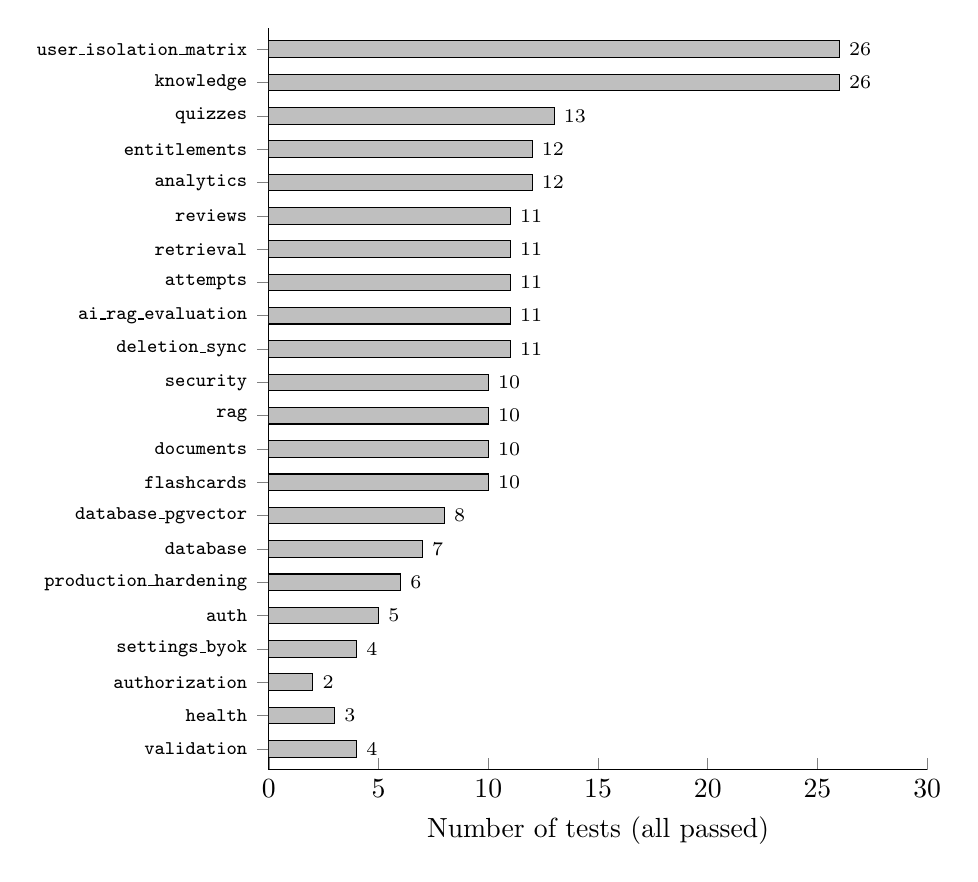
\begin{tikzpicture}
\begin{axis}[
  xbar, width=0.82\textwidth, height=11cm,
  bar width=6pt, xmin=0, xmax=30,
  xlabel={Number of tests (all passed)},
  symbolic y coords={validation,health,authorization,settings\_byok,auth,production\_hardening,database,database\_pgvector,flashcards,documents,rag,security,deletion\_sync,ai\_rag\_evaluation,attempts,retrieval,reviews,analytics,entitlements,quizzes,knowledge,user\_isolation\_matrix},
  ytick=data, y tick label style={font=\scriptsize\ttfamily},
  nodes near coords, nodes near coords style={font=\scriptsize},
  enlarge y limits=0.03, axis lines*=left]
\addplot[fill=black!25, draw=black] coordinates {(4,validation) (3,health) (2,authorization) (4,settings\_byok) (5,auth) (6,production\_hardening) (7,database) (8,database\_pgvector) (10,flashcards) (10,documents) (10,rag) (10,security) (11,deletion\_sync) (11,ai\_rag\_evaluation) (11,attempts) (11,retrieval) (11,reviews) (12,analytics) (12,entitlements) (13,quizzes) (26,knowledge) (26,user\_isolation\_matrix)};
\end{axis}
\end{tikzpicture}
}

%------------------------------------------------------------------
\dgsec{E\quad Additional Diagrams (Appendix E)}
\dg{state_subscription.pdf}{E.1}{State diagram of a subscription in the billing module}
\dg{deployment.pdf}{E.2}{Deployment diagram: the desktop app, the local backend and its
storage on the student's computer, the external AI providers, and the optional container
setup}

%------------------------------------------------------------------
\dgsec{S\quad Full Database Schemas}
\dg{er_saas.pdf}{S.1}{Full schema of the account database \texttt{recall\_saas.db}}
\dg{er_legacy.pdf}{S.2}{Full schema of the per-user study database
\texttt{user\_<id>\_recall.db}}

\end{document}
